\documentclass[../main.tex]{subfiles}
\begin{document}

\subsection*{Exercise 1 – Understanding tire data}
\textbf{Q. Plot the raw data in different graphs, specifically focusing on $\kappa$, $\alpha$, $\gamma$, $\fz$\ and pressure $P$. Comment on what you see. What is, according to you, the main target of these tests?}

        \begin{figure}[ht]
        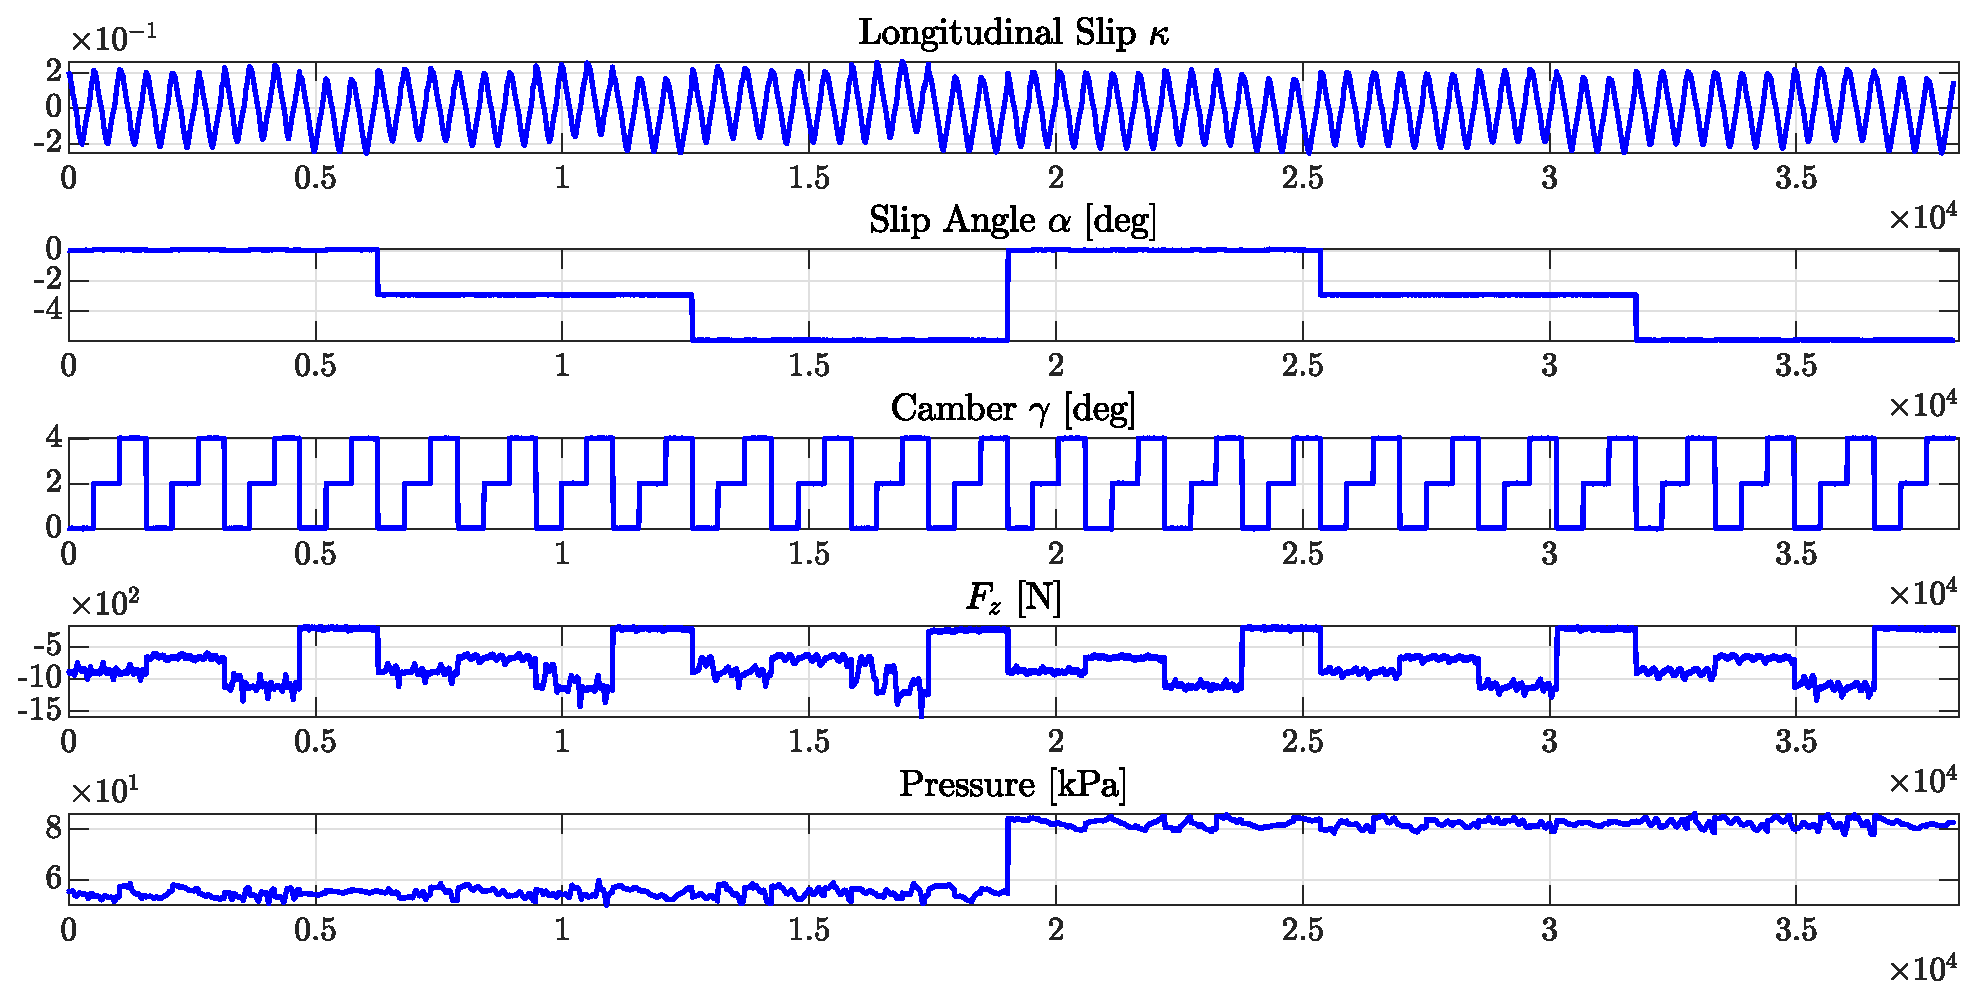
\includegraphics[scale=0.4]{ex2/ex-21.eps}
        \centering
        \caption{raw data}
        \label{rd}
        \end{figure}

From the five plotted variables in Figure \ref{rd}, it appears that the longitudinal slip, slip angle, camber, vertical force, and pressure are all showing repeat patterns. That means that those five variables are controlled to measure and test their effect on the longitudinal force  $\fx$. Note that the longitudinal slip $\kappa$ for each test spanned from 0.2 to -0.2 and then back again to 0.2. The data extracted for the following questions only took the first half of each separate test. Furthermore, only data that had $P$ = 83 kPa were used, because the data seemed noisier with $P$ = 55 kPa, especially with $\fz$\ data.

\textbf{Q. Focus on the data with $\alpha$ =0 and $\gamma$ =0, and plot the curves $\fx$\ vs $\kappa$ for each of the 4 vertical loads $\fz$\ used in the experiments. Plot the 4 curves on the same graph, with different colors. Comment on what you see.}

        \begin{figure}[ht]
        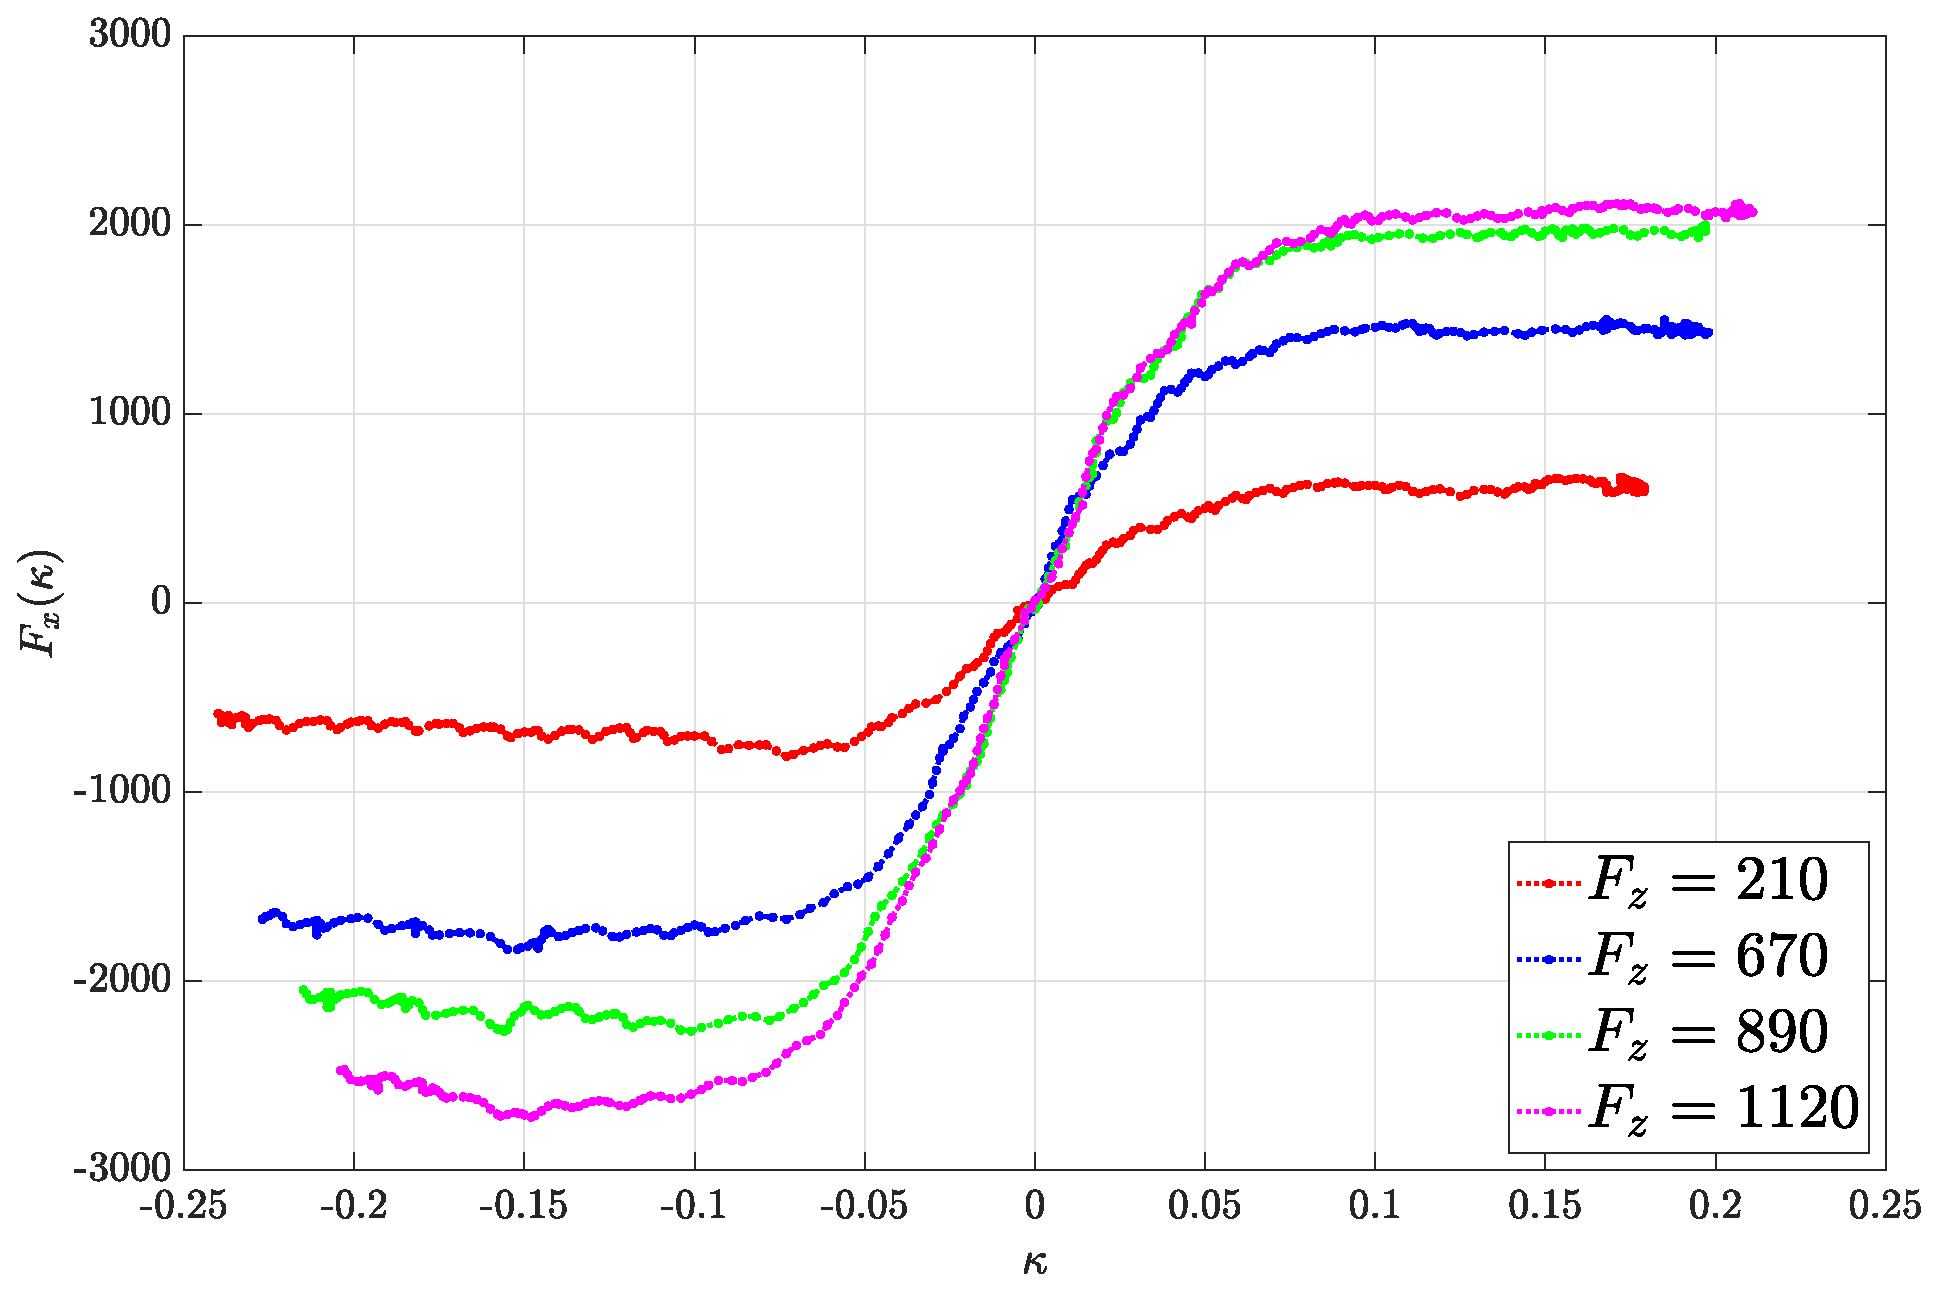
\includegraphics[scale=0.34]{ex2/ex-22.eps}
        \centering
        \caption{$\kappa$ vs $\fx$\ based on vertical force}
        \label{lsvlf}
        \end{figure}

Figure \ref{lsvlf} suggests that the Longitudinal Force $\fx$\ increases with the vertical force $\fz$. There is some dependency on the vertical force. If you double the vertical force, it does not mean the longitudinal force will double. In some parts there is a linear dependency, but in others it is not the case.

\textbf{Q. Focus on the data with $\gamma$ =0 and $\fz$\ = 150 lbf $\approx$ 670N, and plot the curves $\fx$\ vs $\kappa$ for each of the 3 side slip angles $\alpha$ used in the experiments. Plot the 3 curves on the same graph, with different colors. Comment on what you see.}

The Longitudinal Force $\fx$\ in Figure \ref{lsvlfv} shows an inverse relationship with the side slip angle. 
        \begin{figure}[ht]
        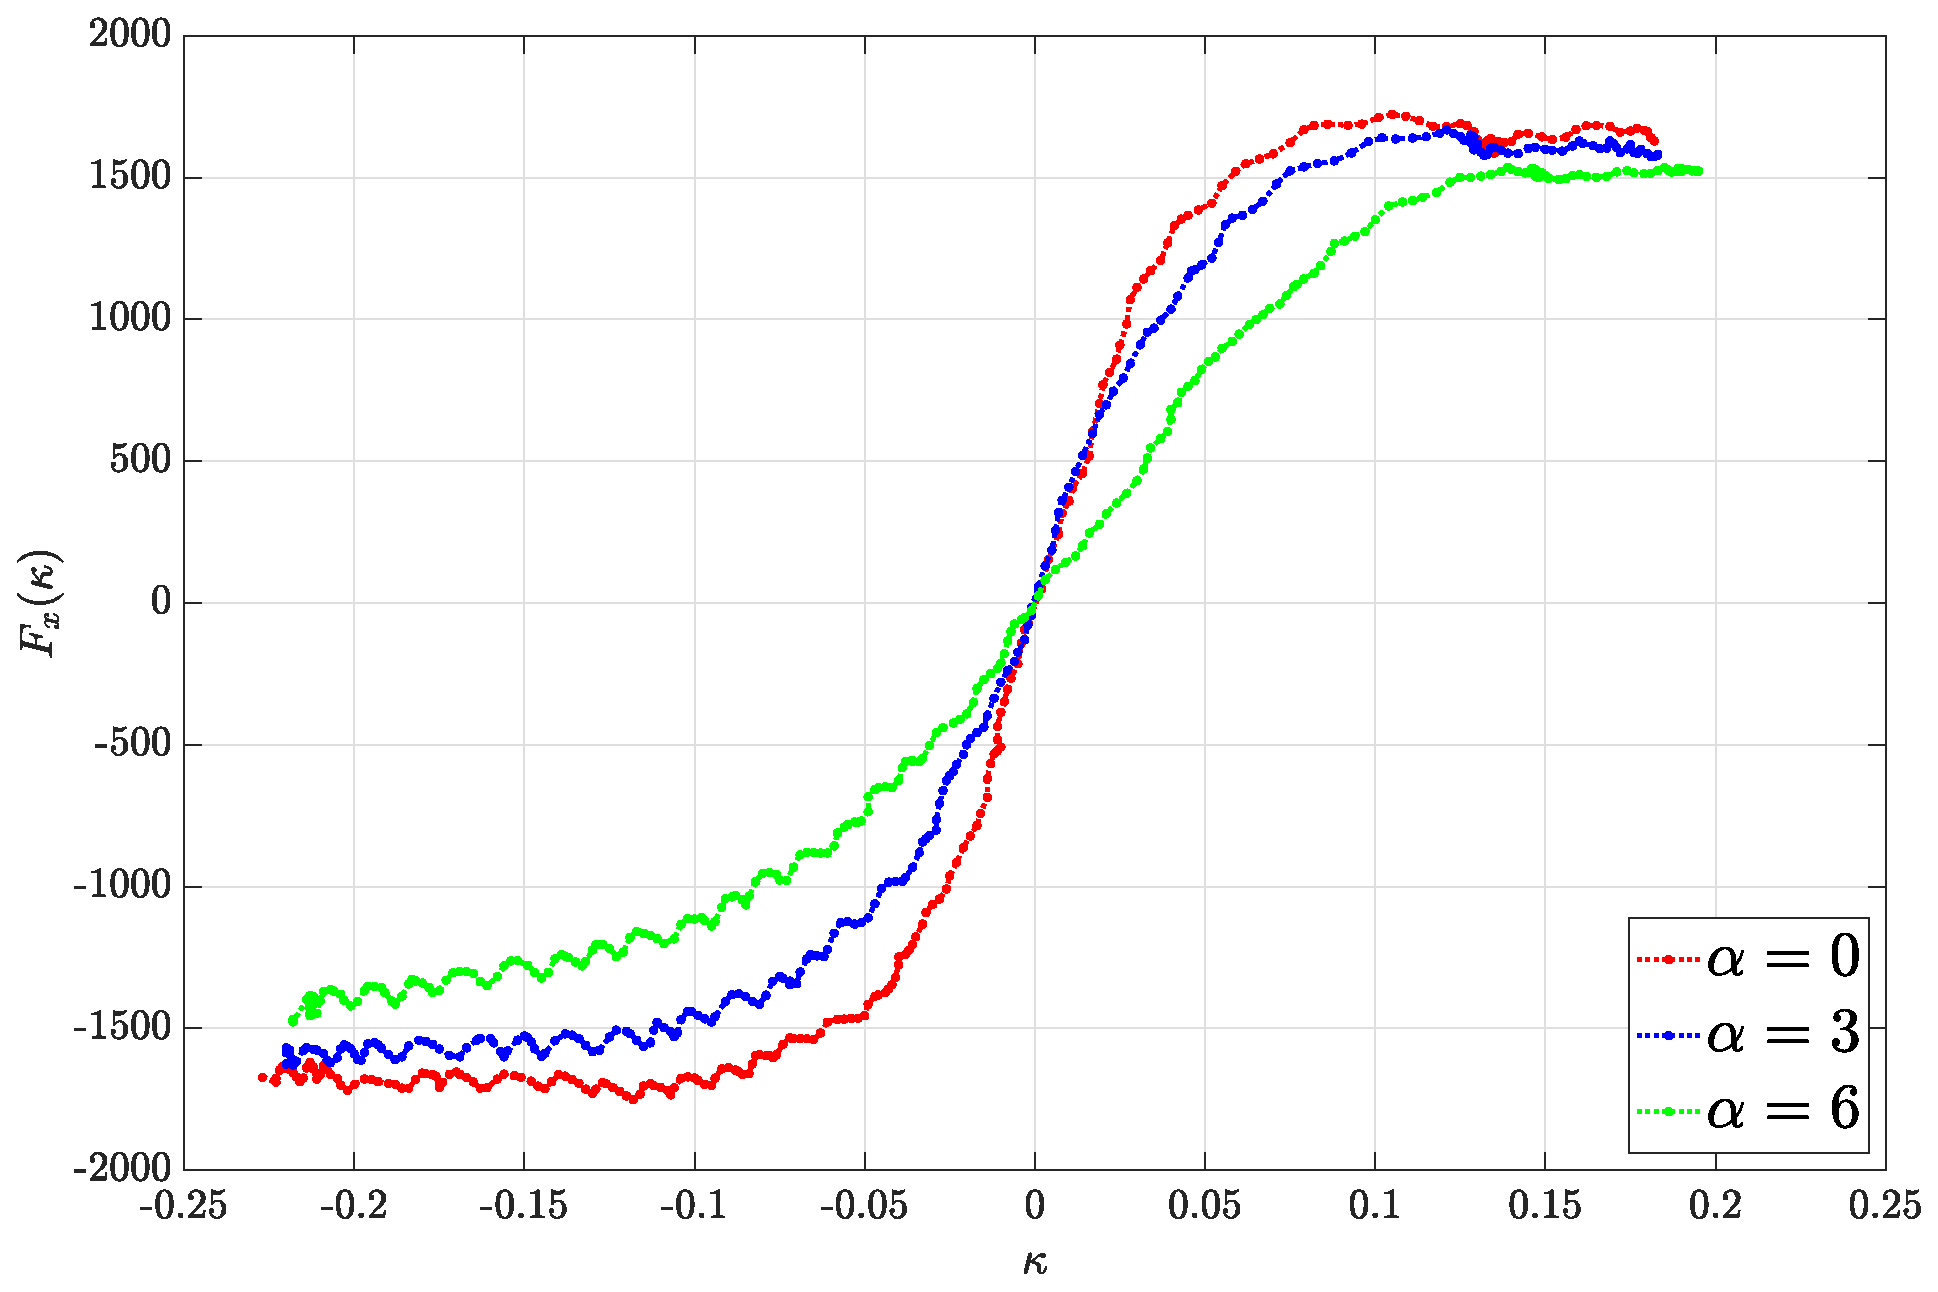
\includegraphics[scale=0.34]{ex2/ex-23.eps}
        \centering
        \caption{$\kappa$ vs $\fx$\ at vertical force = 670 based on slip angle}
        \label{lsvlfv}
        \end{figure}

\subsection*{Exercise 2 - Fitting tire data}

\textbf{Q. First consider the data with $\fz$\ = $\fzz$\ =890N, $\gamma$ =0 and $\alpha$ =0, and fit the coefficients X1 = \{$\pcxo$, $\pdxo$, $\pexo$ , $\pexf$, $\pkxo$, $\phxo$, $\pvxo$\}. Plot the fitted curve $\fx$\ vs $\kappa$ that you obtained in these nominal conditions, together with the raw data.}

        \begin{figure}[ht]
        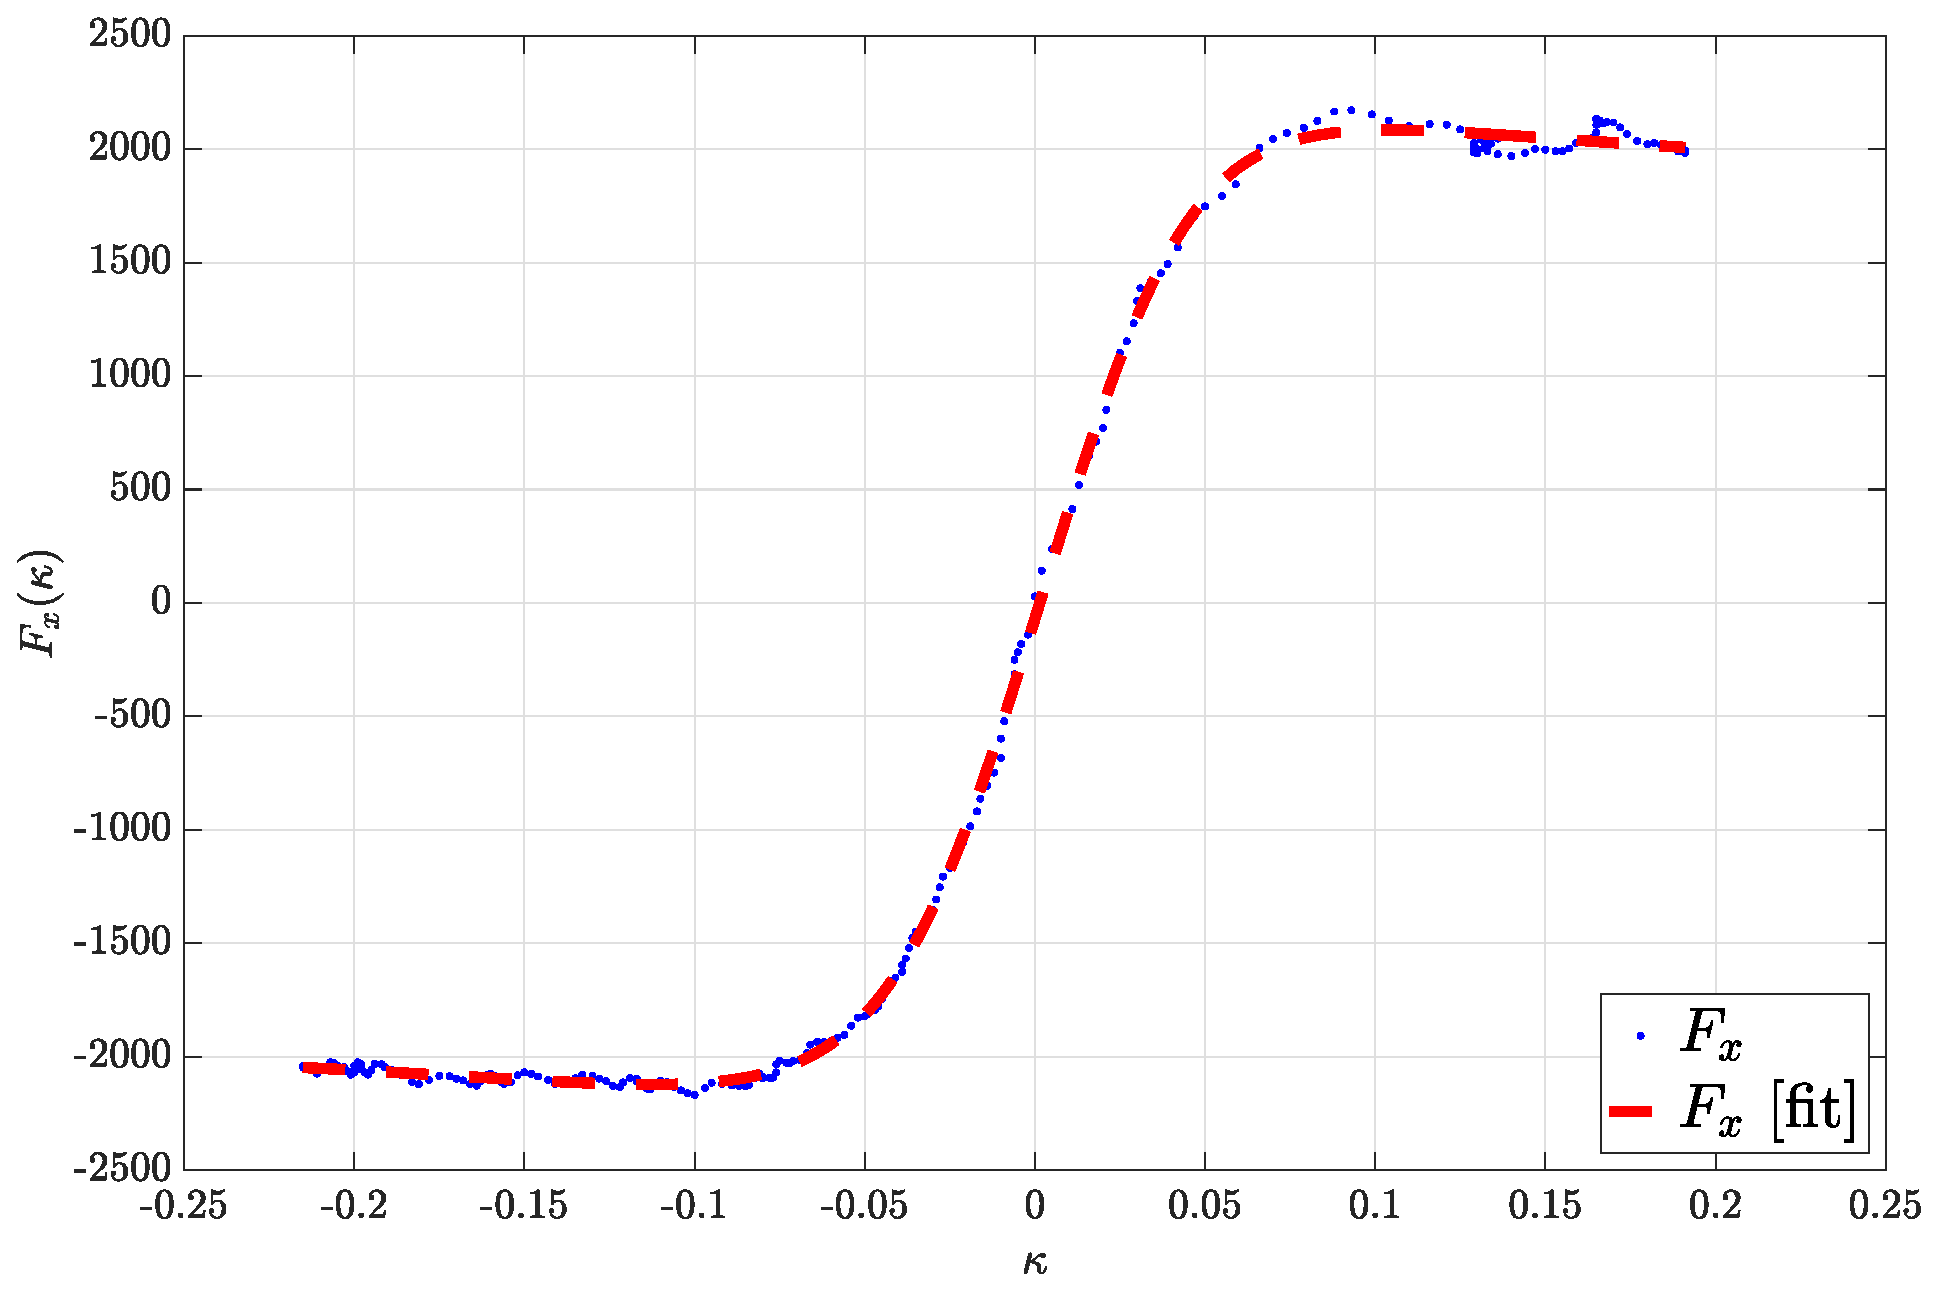
\includegraphics[scale=0.35]{ex2/ex-24.eps}
        \centering
        \caption{Fitted $\fxz$\ after optimizing first 7 parameters compared to test data vs $\kappa$}
        \label{faopt}
        \end{figure}

In Figure \ref{faopt}, the data was filtered based on the following criteria: $\fzz$\ = 890, $\alpha$\ = 0, $\gamma$\ = 0. The first 7 coefficients were optimized using the $fmincon$ function in Matlab. I started with a random coefficients initial guess vector. The initial guess vector has proven to be quite important as running the code multiple times showed a curve that did not fit the data at all, which means the optimizer was stuck at a local minima. However, most of the time the initial guess gave a very good fit that converged to the correct global minima. Later on I optimized the initial guesses to give consistent good fitting results based on trial and error.


\textbf{Q. Now consider the data with the 4 different values of $\fz$, but still $\gamma$ = 0 (and $\alpha$ = 0). This enables the fitting of the parameters: X2 =\{$\pdxt$,$\pext$,$\pextt$,$\phxt$,$\pkxt$,$\pkxtt$,$\pvxt$\}. Plot the fitted and raw curves $\fxz$\ vs $\kappa$ for the 4 values of $\fz$\ and comment the results.}

        \begin{figure}[ht]
        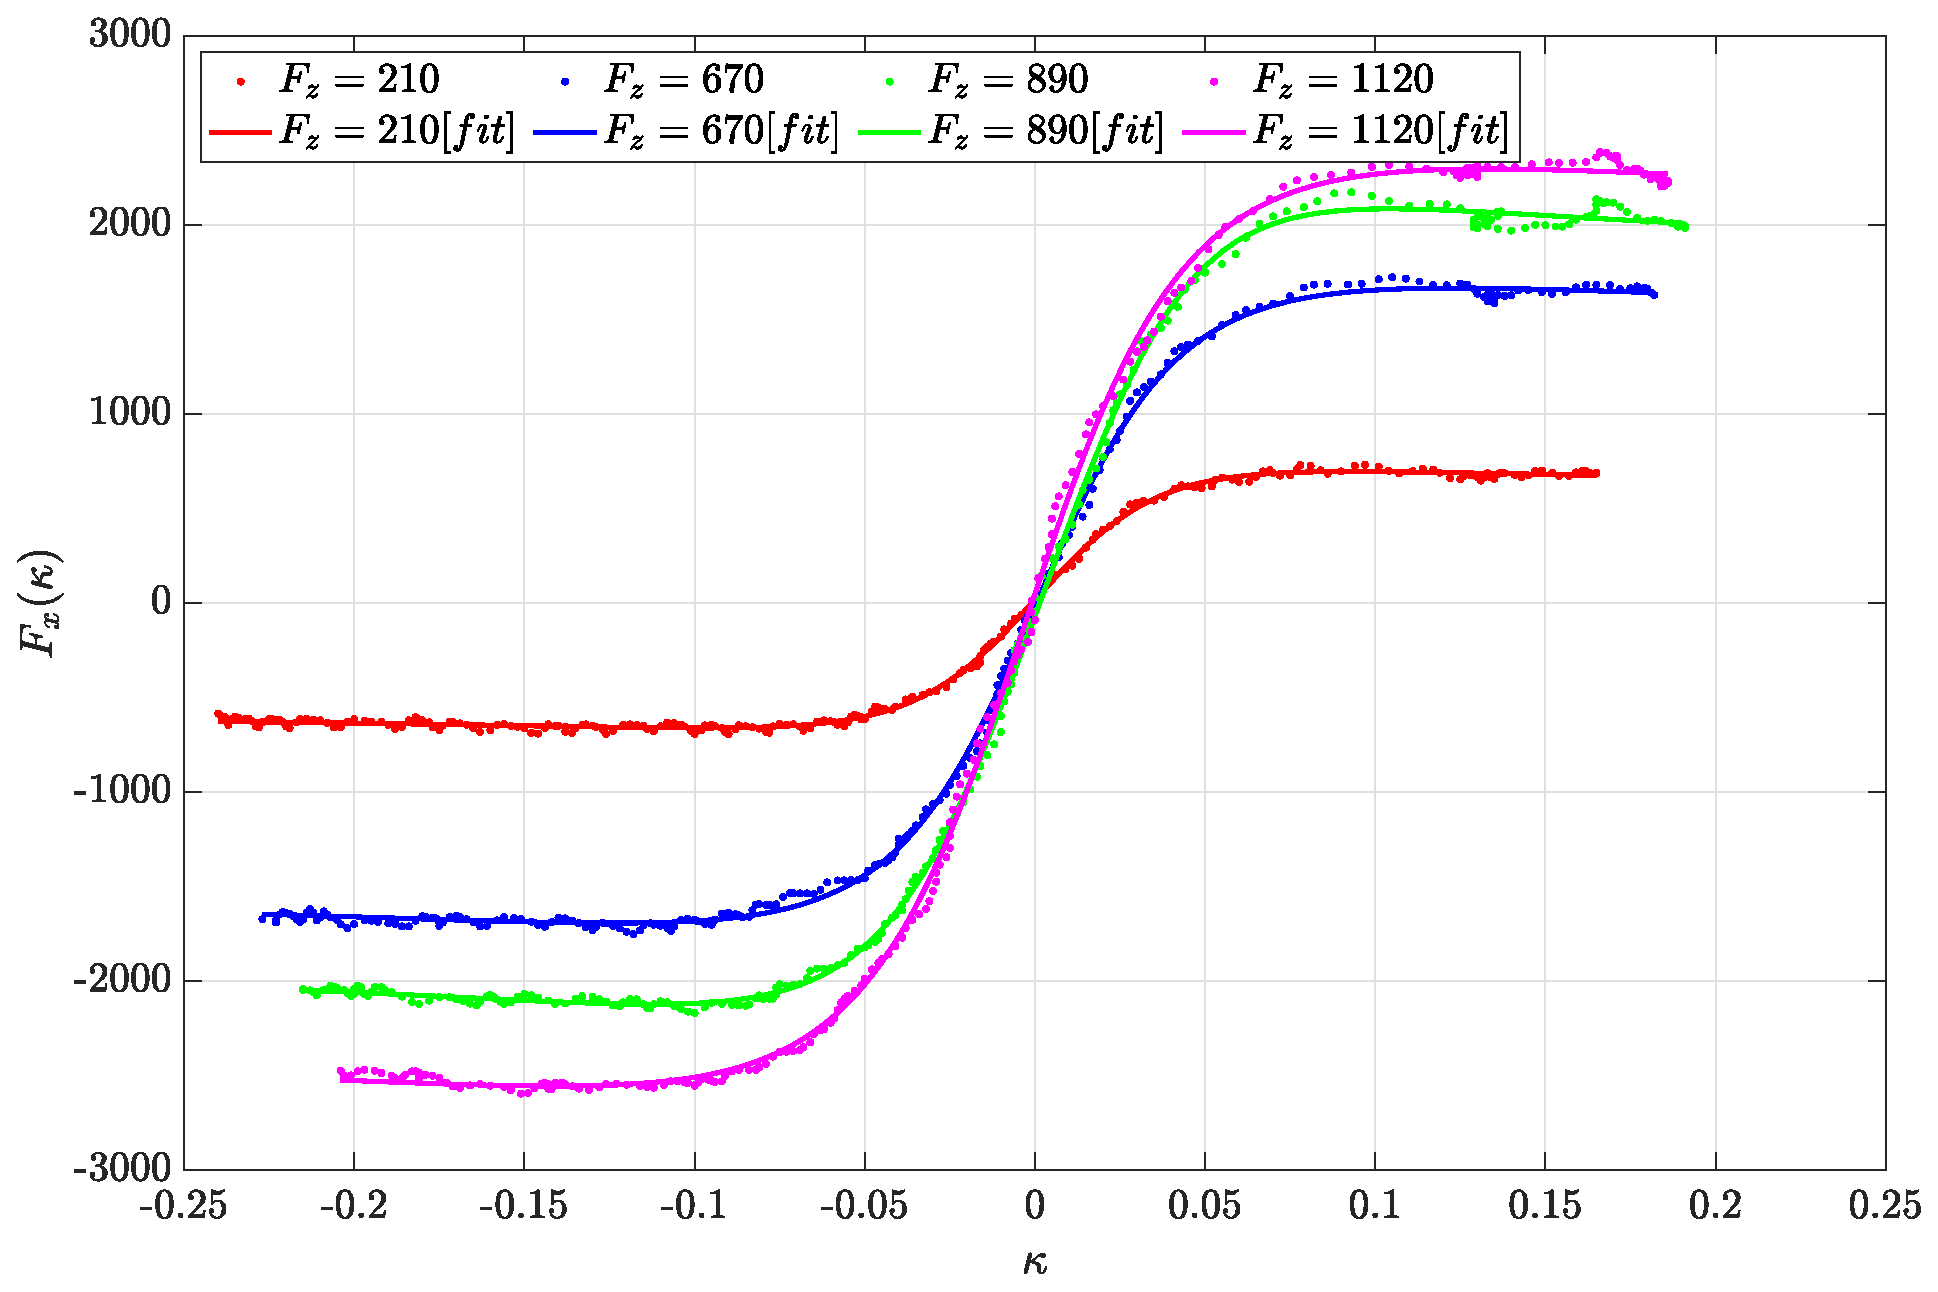
\includegraphics[scale=0.35]{ex2/ex-25.eps}
        \centering
        \caption{Fitted $\fx$\ vs test data after second fitting for each $\fz$}
        \label{ffxtd}
        \end{figure}

The real $\fx$\ data for each separate $\fz$\ are plotted against the output of the second fitting in Figure \ref{ffxtd}. The fitted data appear to match the test data quite well. This means the fitting results are adequate to approximate the longitudinal force $\fx$ for vertical forces $\fz$ that are different from the originally tested one.


\textbf{Q. Now consider the data with the 3 different values of $\gamma$, but with $\fz$\ = $\fzz$\ (and 
$\alpha$ = 0). This enables the fitting of the parameter:
X3 = {$\pdxt$}. Plot the fitted and raw curves $\fxz$\ vs $\kappa$ for the 3 values of $\gamma$ and comment the results.}

        \begin{figure}[ht]
        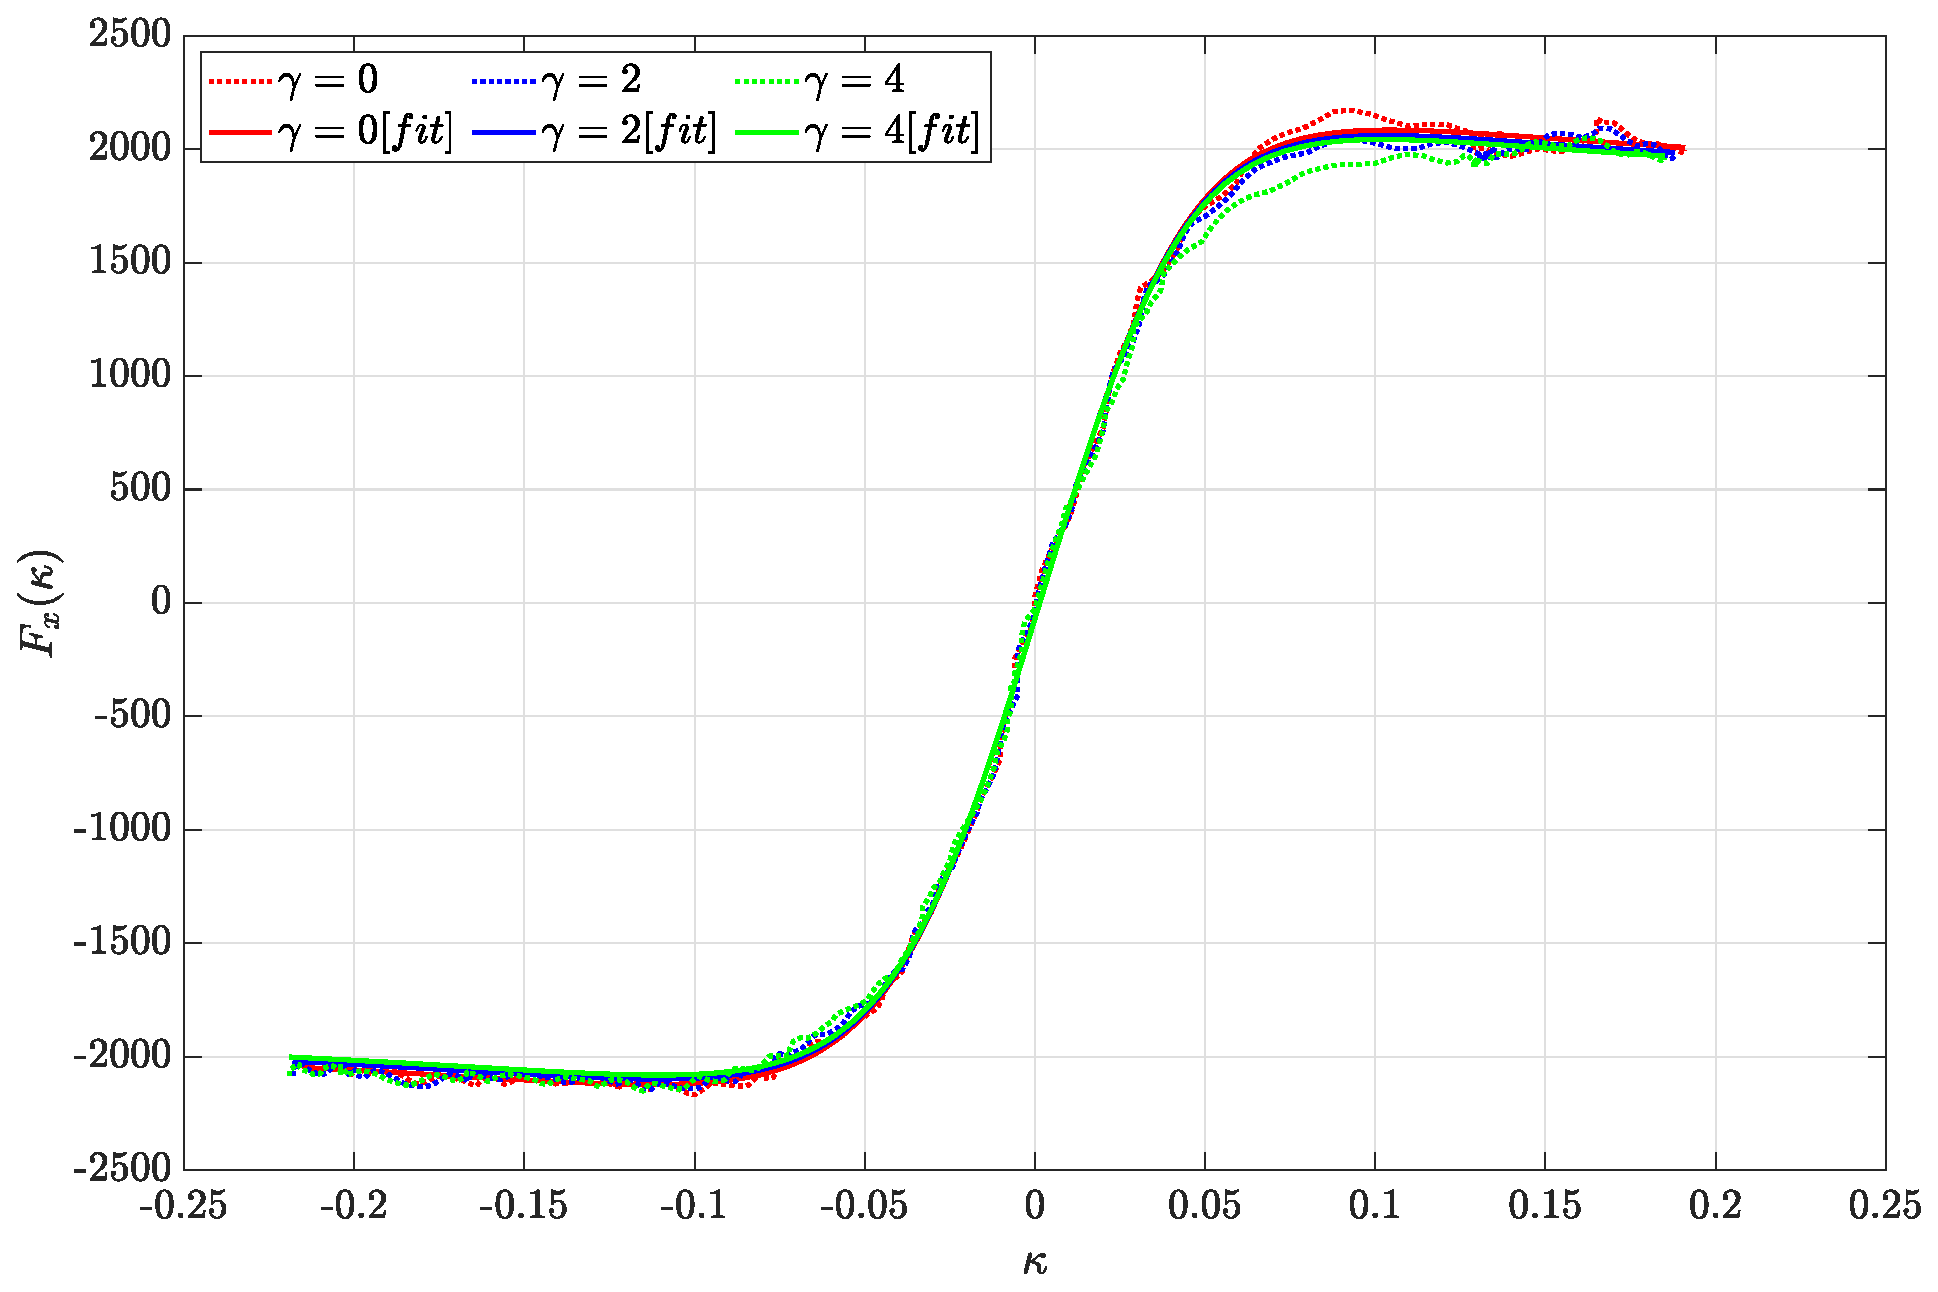
\includegraphics[scale=0.35]{ex2/ex-26.eps}
        \centering
        \caption{Fitted $\fx$\ vs test data after third fitting for each $\gamma$}
        \label{ffvtdg}
        \end{figure}

Figure \ref{ffvtdg} shows the results of the third fitting. The data from $\gamma$ = 0 fits properly as shown previously in Figure \ref{faopt}. However, the fitting on the other $\gamma$ values did not. Trying different initial values for {$\pdxt$} did not yield any better results.
\end{document}